\section*{Zielsetzung}
\label{sec:Zielsetzung}
Das Ziel des in diesem Protokoll beschriebenen Versuchs ist es die Suszeptibilität einiger Seltener-Erd-Elemente zu bestimmen.
\section{Theorie}
\label{sec:Theorie}
\subsection{Die Suszeptibilität paramagnetischer Substanzen}
Die magnetische Flussdichte $\symbf{B}$ hängt bei Anwesenheit von Materie von der magnetischen Feldstärke $\symbf{H}$ und der Magnetisierung $\symbf{M}$ ab:
    \begin{equation}
        \vec B = \mu_0 \vec H + \vec M
    \label{eqn:b}
    \end{equation}
Die Magnetisierung $\symbf{M}$ ist ebenfalls von der magnetischen Feldstärke $\symbf{H}$ abhängig:
\begin{equation}
    \label{eqn:m}
    \vec M = \mu_0 \chi \vec H 
\end{equation} 
Der Proportionalitätsfaktor $\chi$ in \autoref{eqn:m} ist die sogenannte \textbf{Suszeptibilität}.
Generell wird der Paramagnetismus nur bei Atomen, Ionen oder Molekülen beobachtet, die einen nicht verschwindenden Drehimpuls besitzen. Dieses Phänomen entsteht dadurch, dass sich die, mit dem Drehimpuls gekoppelten, magnetischen Momente relativ zum äußeren Magnetfeld ausrichten. Weil die Ausrichtung dieser Momente auch von den thermischen Bewegungen innerhalb des Atoms beeinflusst wird, ist der Paramagnetismus außerdem temperaturabhängig.  
Der Gesamtdrehimpuls $\vec{J}$ eines Atoms setzt sich aus dem Bahndrehimpuls $\vec{L}$ und dem Gesamtspin $\vec{S}$ zusammen.
\begin{equation*}
    \vec{J} = \vec{L} + \vec{S} ,
\end{equation*}
Für die magnetischen Momente gilt: 
\begin{align}
    \vec{\mu_\text{L}} &= - \frac{\mu_\text{B}}{\hbar} \vec{L} \; \text{,} \\
    \vec{\mu_\text{S}} &= - g_\text{S} \frac{\mu_\text{B}}{\hbar} \vec{S}
\end{align}
$\mu_\text{B}=\frac{\hbar e_0}{2m_0} $ beschreibt dabei das Bohrsche Magneton und $g_\text{S}$ das
gyromagnetische Verhältnis.
Aus \autoref{fig:vektor} ergibt sich für $|\vec{\mu_\text{J}}|$:
\begin{equation}
    |\vec{\mu_\text{J}}| = |\vec{\mu_\text{S}}| \cdot \text{cos}\left(\alpha \right) + 
    |\vec{\mu_\text{L}}| \cdot \text{cos}\left(\beta \right)
\end{equation}

\begin{figure}[H]
    \centering
    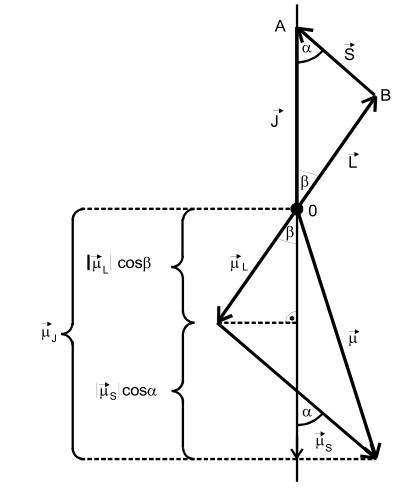
\includegraphics[width=0.5\textwidth]{content/vektoren.JPG}
    \caption{Vektorielle Darstellung der Drehimpulsvektoren und der entsprechenden
    magnetischen Momente \cite{versuchsanleitung}.}
    \label{fig:vektor}
  \end{figure}
\noindent Der Lande-Faktor $g_J$ eines Atoms ist definiert als:
\begin{equation}
    g_J = \frac{3J(J+1) + [S(S+1) - L(L+1)]} {2 J(J+1)}
\end{equation}
Mit dieser Definition gilt für $|\vec{\mu_\text{J}}|$:
\begin{equation}
    |\vec{\mu_\text{J}}| = \vec{\mu_\text{B}} g_J \sqrt{J (J+1)} 
\end{equation}
Bei Seltenen-Erd-Verbindungen resultiert der Gesamtdrehimpuls $\vec{J}$ aus der Anordnung der Elektronen in der unabgeschlossenen 4f-Schale. Diese Anordnung wird durch die \textbf{Hundschen Regeln} beschrieben, die im Folgenden aufgelistet sind:

\begin{itemize}
    \item Die Spins $\vec{s_i}$ summieren sich nach dem Pauli-Prinzip zum maximalen Gesamtspin
    $\vec{S} = \sum \vec{s_i}$ auf.
    \item Die Bahndrehimpulse $\vec{l_i}$ summieren sich nach dem Pauli-Prinzip zum Maximaldrehimpuls 
    $\vec{L} = \sum \vec{l_i}$ auf.
    \item Der Gesamtdrehimpuls beträgt $\vec{J} = \vec{L} - \vec{S}$, wenn die Elektronenschale weniger und
    $\vec{J} = \vec{L} + \vec{S}$, wenn die Schale mehr als halbvoll besetzt ist.
\end{itemize}

\subsection{Messverfahren zur Bestimmung der paramagnetischen Suszeptibilität}
\label{sec:mess}
Bei der Messung der paramagnetischen Suszeptibilität macht man sich zu Nutze, dass sich die Induktivität einer Spule ändert, wenn ein Material in sie eingeführt wird. Die Induktivität im Vakuum $L = \mu_0 \frac{n^2 F}{l}$ ändert sich in Materie zu:
\begin{equation}
    L_\text{M} = \mu_0 \frac{n^2 F}{l} + \chi \mu_0 \frac{n^2 Q}{l} 
\end{equation}
Wobei $n$ die Windungszahl, $l$ die Länge, $F$ der Querschnitt der Spule und $Q$ der Querschnitt der Probe ist.
Als Differenz der Induktivitäten ergibt sich also: 
\begin{equation}
    \symup{\Delta} L = \mu_0 \chi Q \frac{n^2}{l} 
\end{equation}

\begin{figure}[H]
    \centering
    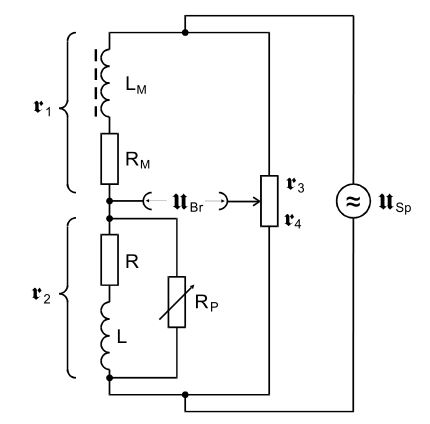
\includegraphics[width=0.5\textwidth]{content/bruecke.JPG}
    \caption{Brückenschaltung zur Suszeptibilitätsmessung \cite{versuchsanleitung}.}
    \label{fig:bruecke}
  \end{figure}
\noindent Für die Suszeptibilitätsmessung wird eine Brückenschaltung nach \autoref{fig:bruecke} verwendet. Für den Betrag der Brückenspannung einer solchen Schaltung ergibt sich:
\begin{equation}
U_\text{Br} = \frac{\omega \symup{\Delta} L}{4} \frac{1}{\sqrt{R^2 + {\omega}^2 L^2 }} U_\text{Sp}
\end{equation}
Hier können die bereits beschriebenen $L$  und $\symup{\Delta} L$ eingesetzt werden und man erhält:
\begin{equation}
U_\text{Br} = \frac{\omega \mu_0 \chi n^2 Q}{4l} \frac{1}{\sqrt{R^2 + {\omega}^2(\mu_0 \frac{n^2}{l}F)^2}} U_\text{Sp}
\end{equation}
Die Abgleichbedingung für die Schaltung ohne Probe ist
\begin{equation}
    r_1 R_4 = r_2 R_3 .
\end{equation}
Nach Einfügen der Probe ändert sich $R_3$ zu $R'_3 = R_3 + \symup{\Delta}R$ .
Für $\symup{\Delta}R$ ergibt sich nach Umformungen:
\begin{equation}
    \symup{\Delta}R = \frac{R_3 (L_\text{M} - L)}{L + L_\text{M}} 
\end{equation}
Hier können $L$ und $L_\text{M}$ eingesetzt werden und es ergibt sich schließlich für die Suszeptibilität $\chi$:
\begin{equation}
    \label{eqn:chi}
    \chi = 2 \frac{\symup{\Delta}R}{R_3} \frac{F}{Q}
\end{equation}

\subsection{Unterdrückung von Störspannungen}
Bei der Messung der Brückenspannung stellen die immer auftretenden Störspannungen ein Problem dar. Um dieses Problem zu beheben kann ein Selektivverstärker, der als Frequenzfilter dient, genutzt werden. die typische Form der Filterkurve eines solchen Verstärkers ist in \autoref{fig:filterkurve2} dargestellt.
\begin{figure}[H]
    \centering
    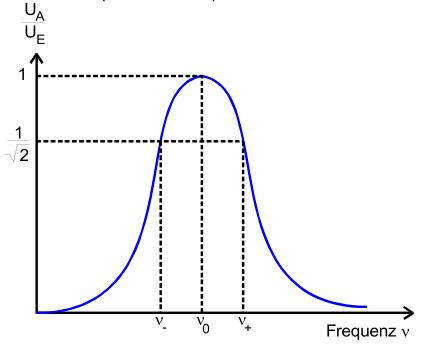
\includegraphics[width=0.5\textwidth]{content/filterkurve.jpg}
    \caption{Filterkurve \cite{versuchsanleitung}.}
    \label{fig:filterkurve2}
\end{figure}
\noindent Die Güte $Q$ ist ein Maß für die Qualität des Filters und kann nach 
  \begin{equation}
    \label{eqn:güte}
    Q = \frac{\nu_0}{\nu_+ - \nu_-}
\end{equation}
berechnet werden. Dabei ist $\nu_0$ die Durchlassfrequenz des Selektivverstärkers und $\nu_+$ und $\nu_-$ sind die Frequenzen,
bei denen $\frac{U_\text{A}}{U_\text{E}}$ auf $\frac{1}{\sqrt{2}}$ gefallen ist.
